\documentclass{article}
\usepackage{graphicx} % Required for inserting images
\usepackage{amssymb}
\usepackage{bm}
\usepackage{bbm}
\usepackage{hyperref}
\usepackage{amsmath}
\usepackage{algorithm}
\usepackage{algpseudocode}
\usepackage{tikz-cd}
\usepackage{float}


\title{Next token prediction}
\author{Jake Feldman Starosta}
\date{June 2026}

\begin{document}

\maketitle

\section{Introduction}
We want to model feature-label pairs $(\bm{x}^k, y^k)$ in a dataset $\mathcal{D}$, where $y^k$ is the empirical conditional probability measure given that features are $N$th-order Markov. 

\subsection{Notation:}
\begin{itemize}
\item $S \subset \mathbb{R}^d$ - individual token embedding space 
\item $\mathcal{N} = \{1, ..., N\} $ - token index of $N$th-order Markov chain
\item $x^{i,k} \in S$ - individual token embedding
\item $\tilde y^k \in S$ - target token embedding
\item $\bm{x}^k = (x^{1, k}, \dots, x^{N, k}) \in S^N$ - training sample/feature vector
\item $p_i \in PE_N = \{1, \dots, N\}$ - positional encoding of token $i$ (change to $\mathcal{N}$?)
\item $X^{i,k} = (x^{i, k} , p_i) \in \mathbb{X} = S\times PE_N$ - feature with token and  positional encoding
\item $U = (W, A, b, Q, K, V) \in \mathbb{U}$ - actions/model weights
\item $\mathcal{T} = \{0, \dots, T\}$ - time index for $T \in \mathbb N$


\end{itemize}

The difference between this problem and the original paper's \cite{akman2026optimal} formulation is that our final distribution has 1. no positional information and 2. lives in a different space to our input. 


\section{Dataset}

We begin by constructing a generally non-Markovian process $\{Y_r\}_{r \in \mathbb{Z_+}}$ on $S^\mathbb{Z_+}$ parameterized by $\xi \in [0,1]$, a parameter controlling its Markovian characteristic. We define an $N$th order Markov chain $\{Z_r\}_{r \in \mathbb{Z_+}}$ on $S^\mathbb{Z_+}$ with transition kernel 
$$P(Z_r\in A|Z_{[0, r-1]}) = P(Z_r\in A|Z_{[\max(0, r-N), r-1]})$$
and a stochastic process $\{V_r\}_{r \in \mathbb{Z_+}}$ on $S^\mathbb{Z_+}$
where $V_r \overset{\text{iid}}\sim \mu$ for some $\mu \in P(S)$ and all $r \in \mathbb Z _+$. Then our desired process is given by $Y_r = h(Z_r, V_r, \xi)$ for $r \in \mathbb Z _+$, where $h$ can be taken, for instance, as
$$h(Z_r, V_r, \xi) = \xi \cdot Z_r + (1-\xi) \cdot V_r.$$

% We begin by constructing a generally non-Markovian process $\{Z_r\}_{r \in \mathbb{Z_+}}$ on $S^\mathbb{Z_+}$ parameterized by $\xi \in [0,1]$, a parameter controlling its Markovian characteristic. For all Borel $A \subset S$, we define an $N$th order Markov transition probability
% $$P_1(z_t\in A|z_{[0, t-1]}) = P_1(z_t\in A|z_{[\max(0, t-N), t-1]})$$
% and a non-Markovian transition probability 
% $$P_2(z_t\in A|z_{[0, t-1]}) = P_2(z_t\in A|z_{[0, \max(0, t-N-1)]}).
% $$ 
% We then define the transition probability $P$ of $\{z_r\}$ as 
% $$ P(z_t\in A|z_{[0, t-1]}) = \xi \cdot P_1(z_t\in A|z_{[\max(0, t-N), t-1]}) + (1 - \xi) \cdot P_2(z_t\in A|z_{[0, \max(0, t-N-1)]}).
% $$

% Note that $\{z_r\}$ is an $N$th order Markov chain if and only if $\xi = 1$  .

% Note to self: Do we want P to be ergodic? If so, it may be difficult if P2 has increasing context. Might want to cap P2 to be markovian of order 2N, prove ergodicity on that, then bring it back to show that it holds for P. 

We generate $\tilde K$ sequences of length $N+1$ from the process $\{Y_r\}$. We split each sequence into a training pair by taking $\bm{x}^k = (x^{1, k}, \dots, x^{N, k})$ as the first $N$ elements of the sequence and $\tilde y^k$ as the last element, for $k \in \tilde {\mathcal{K}} = \{1, \dots , \tilde K\}$. We aggregate these prompts to an initial single state-labeled dataset, given by 
$$\tilde D = \{(\bm{x}^k, \tilde y^k):k \in \tilde {\mathcal{K}} \} \in (S^N \times S)^{\tilde K}$$
where $\bm{x}^k$ is the feature vector and $\tilde{y}^k \in S$ is the target token embedding. The initial dataset $\hat D$ has training pairs indexed by $\tilde {\mathcal{K}}$, with possibly some duplicate feature vectors, i.e., $\bm{x}^j = \bm{x}^l$ for $j\neq l$, and $j, l \in \tilde {\mathcal{K}}$. 

We construct a new dataset $D$ from $\tilde D$ with unique feature vectors and labels as probability measures instead of individual token embeddings. 
We index the unique feature vectors with $\mathcal{K} = \{1, \dots, K\}$, picking one representative index from $\tilde {\mathcal{K}}$ for each unique feature vector. For $k \in \mathcal{K}$, we define the empirical measure $y^k \in P(S)$ conditioned on $\bm{x}^k$ as  
$$y^k = \frac{
\sum_{l=1}^{\tilde {K}} \delta _ {\tilde y^l} \mathbbm{1}_{\{\bm{x}^l = \bm{x}^k\}}
}{\sum_{l=1}^{\tilde {K}} \mathbbm{1}_{\{\bm{x}^l = \bm{x}^k\}}
}
.$$

Then $D = \{(\bm{x}^k, y^k):k \in \mathcal{K}\} \in (S^N \times P(S))^K$ has unique training samples $\bm{x}^k$, with labels $y^k$ as empirical probability measures. Note that the denominator is non-zero since it is the count of samples in $\hat D$ with feature vector $\bm{x}^k$.

A distinction between this dataset construction and that of most large language models (LLMs) is that here we exclude elements of generated process appearing after the target label at the dataset level, whereas most current pre-trained LLMs use the technique of masking \cite{devlin2019bertpretrainingdeepbidirectional} during training. \cite{zhao2024analysing}

\section{Transformer Dynamics}
We avoid positional encoding in the first lift. Encoding position separately from the state itself is somewhat superfluous: embeddings are useful precisely because attention is inherently position-agnostic (or permutation-equivariant \cite{geshkovski2025mathematical}) and requires position information embedded at the state level. Mathematically, $\text{lifted-attn}((p, x)) := (p, attn(x))$ is insufficient. We require $\text{lifted-attn}((p, x)) := (p, attn(g(p, x)))$, for some embedding function $g$.

To depict how position is used in early transformers (now it's done at the attention matrix level \cite{barbero2024round}), this requires generating a token from a static 'vocabulary' and then embedding it with positional information. 

For simplicity and to preserve the notation from the previous paper, we say that $S$ is the vocabulary, which has the same shape as $\mathbb{X}$, the token embedding space (which we can change in the future). Then, we encode position $p \in PE_N$ into $x \in S$ via $g:S\times PE_N \to \mathbb{X}$, where we can trivially take $g(x, p) = x$, for instance. From now on, we assume that positional information is embedded in $x^{i,k}$ via $g$ for $i \in \mathcal N$ and $k \in \mathcal K$. 

We define the particle flow function $f: \mathbb X \times \mathbb U \times P(\mathbb X) \to \mathbb X$ for all $x \in \mathbb X$, $U = (W, A, b, Q, K, V)$, and $\mu \in P(\mathbb X)$ by 
$$
f(x, U, \mu) := W \sigma(Ax + b) + \frac{\int _ \mathbb{X} \mu(dz)e^{\beta \langle Qx, Kz \rangle} Vz}{\int _ \mathbb{X} \mu(dz)e^{\beta \langle Qx, Kz \rangle} }
$$
for a sharpening parameter $\beta \geq 0$. 

For our realization, we take $x ^{i, k}_t \in \mathbb X$, $U_t \in \mathbb U$, and $\mu _t ^k := \frac{1}{N} \sum_{i=1}^N \delta _{x^{i, k}} \in P(\mathbb X)$ for $i \in \mathcal N$, $k \in \mathcal K$, and $t \in \mathcal T$. The particle flow function represents a single token embedding progressing through time, such that
\begin{align*}
f(x ^{i, k}_t, U_t, \mu _t ^k) &= W_t \sigma(A_t x ^{i, k}_t + b_t) + \frac{\int _\mathbb X \mu _t ^k(dz)e^{\beta \langle Q_t x ^{i, k}_t, K_t z \rangle} V_t z}{\int _ \mathbb X \mu _t ^k(dz)e^{\beta \langle Q_t x ^{i, k}_t, K_t z \rangle} }\\
&=W_t \sigma(A_t x ^{i, k}_t + b_t) + \frac{\sum _{j = 1}^N e^{\beta \langle Q_t x ^{i, k}_t, K_t x^{j, k}_t \rangle } V_t x^{j, k}_t}{\sum _{l = 1}^{N} e^{\beta \langle Q_t x ^{i, k}_t, K_t x^{j, k}_t \rangle }} = x^{i, k}_{t + 1}
\end{align*}

%Note to self: It seems that measures are not required, except at the end for comparing $\bm x^k_T$ against the measure-valued label $y^k$. All internal transformer dynamics (feed forward, attention) are deterministic, and currently all intermediate measures are turned into Dirac measures immediately. However, I assume it allows us to use McKean-Vlasov structures.

% We pair each $x^{i, k}$ in $\bm{x}^k = (x^{1, k}, \dots, x^{N, k})$ with its positional encoding $PE_N$ to create a superstate $X^{i, k} = ( p_i, x^{i, k})$ for $i \in \mathcal{N} := \{1, \dots, N\}$. We aggregate these to a position-encoded feature vector $X^k = (X^{1, k}, \dots X^{N, k})$ for all $k \in \mathcal{K}$. We construct an empirical measure $\mu^i_t \in P(\mathbb{X})$, encoding each particle state and position information. It evolves with a deterministic pushforward $\Phi: P(\mathbb{X})\times \mathbb U \to P(\mathbb{X})$ where $\Phi (\mu , U) = \mu \circ f(\cdot , U, \mu)$ for $T$ layers indexed by $\mathcal{T}$. 


We then aggregate all $\mu^i_t$ to an ensemble $((\mu^1_t, ... , \mu^K_t))_{t \in \mathcal{T}}=(\vec \mu_t)_{t \in \mathcal{T}}$ with transition kernel $\eta : P(\mathbb{X})^K \times \mathbb U\to P(P(\mathbb{X}))^K$, where $\eta (\cdot|\vec\mu, U) = \delta _{(\bm{\Phi} (\vec \mu, U))}(\cdot)$ and $\bm{\Phi} : P(\mathbb{X})^K\times \mathbb U \to P(\mathbb{X})^K$ with $\Phi$ applied pointwise to each $\mu^i_t$. 

This defines a MDP on the state space $P(\mathbb{X})^K$ having elements $(\vec \mu_t)_{t \in \mathcal{T}}$, with action space $\mathbb U$, transition kernel $\eta$ and the cost $c$ shown below.

We aim to minimize the following loss functional for a policy $\gamma$:

$$
V(D, \gamma) =  \frac{1}{K}\sum _{k = 1}^K W_{2}(\nu^k ,y^k)^2 
$$

We define $\nu^k := \delta_{x^{k, N}_{T, \gamma}}$, where $x^{k, N}_{T, \gamma}$ starts at $x^{k, N}_{0, \gamma} \in S$ belonging to the ensemble probability measure $\mu^k$ evolving according to $\bm{\Phi}$ which takes actions from $\gamma$. We have

$$W_2(P, Q) = \inf _{\pi \in \Pi (P, Q)} \int _{S \times S} \pi(dx, dy) c(x, y)^2$$

with the cost function 

$$ c(x, y) =  \sqrt{||x-y||_2^2}.$$

For our loss, we only compare the probability measure of the last position ($p_N = \frac{N}{N} = 1$) in the output vectors to our label. This is also a trick used in practice in transformer fine-tuning, where features and labels are separated this way (see equation 3 of \cite{radford2018improving}). 

Although this works for training, we're not actually predicting a distribution. We're just predicting a token embedding, and comparing it to the empirical conditional probability measure. 

\section{Quantization}

We select parameters $l, m, n$ to quantize the above MDP into MDP$^{(l, m, n)}$ as follows: we quantize the values of the probability measure on the state space with $l$, the state space itself with $n$, and the action space with $m$. 
We quantize the token embedding space as $S_n$ such that given $x \in S$, we can find some $s \in S_n$ that satisfies
$$|x - s| < \frac{1}{n}$$
which, due to the compactness of $S$, exists and is finite for all $n$. Similarly, due to the compactness of $\mathbb{U}$, we quantize the action space finitely as $\mathbb{U}_m$ so that given $U \in \mathbb{U}$,
$$||U - \hat U||_F < \frac{1}{m}$$
for some $\hat U \in \mathbb{U}_m$, where $||\cdot ||_F$ is the product Frobenius norm. 

Let $\mathbb{X}_n := PE_N \times S_n$ and define the set of quantized probability measures on $\mathbb{X}_n$ as 
$$\mathcal{P} ^{(l)}(\mathbb X_n) = \{(p_a)_{a = 1}^{|\mathbb X_n|}: p_a \in \frac{1}{l} \mathbb{N}_0, \sum_{a = 1}^{|\mathbb X_n|} p_a = 1\}.$$

We define the quantizers $Q_n : \mathbb{X} \to \mathbb{X}_n$ mapping $x \in \mathbb{X}$ to the closest point in $\mathbb{X}_n$ while preserving position, and $R_l : \mathcal P(\mathbb X _n) \to \mathcal P^{(l)}(\mathbb X _n)$ mapping $\hat \mu \in \mathcal P(\mathbb X _n)$ to the closest element in $\mathcal P^{(l)}(\mathbb X _n)$. 

The quantized deterministic ensemble pushforward $\bm \Phi^{(l, n, m)}$ maps $\mathcal P(\mathbb{X}_n)^K\times \mathbb U_m \to \mathcal P(\mathbb X_n)^K$ by quantizing and applying the single-measure pushforward $\Phi ^{(n)}: \mathcal P(\mathbb X_n) \times \mathbb U\to \mathcal P (\mathbb X_n)$ point-wise. It induces the transition kernel $\eta ^{(l, n, m)} : \mathcal P(\mathbb{X}_n)\times \mathbb U_m \to \mathcal P(\mathcal P(\mathbb X_n))$. This characterizes $\text{MDP}^{(l, n, m)}$ with a state space $\mathcal P(\mathbb{X}_n)^K$, action space $\mathbb U_m$, transition kernel $\eta^{(l, n, m)}$ and the same cost $c$ as MDP.

For $\hat \mu, \hat \nu \in P(S_n)$, we define the measure-level cost as 
$$\hat W_2 (\hat \mu, \hat \nu) = \min _{\hat \pi \in \Pi (\hat \mu, \hat \nu)} \sum _ {\hat x \in S_n}  \sum _ {\hat y \in S_n} \hat \pi (\hat x, \hat y)c(\hat x, \hat y)^2$$

where $$\hat \Pi (\hat \mu, \hat \nu) = \{\hat \pi \in S_n \times S_n : \hat \pi (a,b) \geq 0, \sum _ {a \in S_n} \hat \pi (a, b) = \hat \nu, \sum _ {b \in S_n} \hat \pi (a, b) = \hat \mu\}.$$ 

Our terminal loss functional for $\text{MDP}^{(l, n, m)}$ is given as 
$$\hat V(D, \hat \gamma) = \frac{1}{K}\sum _{k = 1}^K \hat W_{2}(\hat \mu^{k, N}_T ,\hat y^k)^2$$

where $\hat \mu^{k, N}_T := \delta_{\hat x^{k, N}_{T, \gamma}}$ and $\hat y^k := R_l(y^k)$. Our prediction $\hat x^{k, N}_{T, \hat \gamma}$ is initialized at $\hat x^{k, N}_{0, \hat \gamma} \in S_n$ belonging to the ensemble probability measure $\hat \mu^k$ evolving according to $\bm{\Phi}^{(l, n, m)}$ which takes actions from $\hat \gamma$. 

Note that this loss functional is sufficient for training (as it uses all our prediction information), but does not necessarily translate to performance. Specifically, taking a small $l$ may artificially decrease loss without gaining performance due to coarseness. 

For a given dataset $D$, we pose the dynamic programming equations for $\text{MDP}^{(l, n, m)}$ as follows
$$
\begin{aligned} & \mathfrak C _ {l, n, m, T} (\hat {\bm \mu}) := \frac{1}{K}\sum _{k = 1}^K \hat W_{2}(\hat \mu^{k, N}_T ,\hat y^k)^2\\
&\mathfrak C _ {l, n, m, t} (\hat {\bm \mu}) := \min_{U \in \mathbb U_m} \sum _{\hat{\bm \mu}_{t +1} \in P^{(l)}(\mathbb X_n)^K} \eta^{(l, n, m)}(\hat{\bm \mu}_{t + 1}| \hat{\bm \mu}_t, U)\mathfrak C _ {l, n, m, t + 1} (\hat{\bm \mu}_{t + 1})\\
&\phantom{\mathfrak C _ {l, n, m, t} (\hat {\bm \mu})}= \min_{U \in \mathbb U_m} \mathfrak C _ {l, n, m, t+1} (\bm \Phi ^{(l, n, m)}(\hat {\bm \mu}, U))
\end{aligned}
$$

for all $\hat{\bm \mu} = (\hat \mu ^1, \dots \hat \mu ^K)\in \mathcal P^{(l)}(\mathbb X _n)^K$ and $t \in \mathcal T$. The last equality is due to the deterministic nature of $\bm \Phi ^{(l, n, m)}$.

Note for myself: do we not need to discretize the second one? Not that it should change the policy, but that we don't even have a clean space defined. Also, because the domain of integration isn't continuous. 

\begin{figure}
    \centering
    \begin{tikzcd}[row sep=3em, column sep=3em]
    P(\mathbb{X}) 
      & P(\mathbb{X}_n) \arrow[r, "R_l"] 
      & P^{(l)}(\mathbb{X}_n) 
      \\
    \mathbb{X} \arrow[u, "\text{lift as } \text{probability measure}"] \arrow[r, "Q_n"]
      & \mathbb{X}_n \arrow[u] 
      & 
      \\
    S \arrow[u, "\text{lift with } P_{EN}"] \arrow[r, "\text{quantize}"] 
      & S_n \arrow[u]
      & \\
    \end{tikzcd}
    \caption{Two-stage State Quantization}
    \label{fig:quantization}
\end{figure}


\section{Algorithm}

\begin{algorithm}
\caption{Next Token Prediction with Dynamic Programming}
\begin{algorithmic}[1]

\State \textbf{Input:} data set $\tilde D = \{(\bm x ^k, \tilde y^k)\}_{k=1}^ {\tilde K}$, horizon $T$, quantization levels $(l, n, m)$

\State Construct state grid $S_n$ from $S$ and for $(p,x) \in \mathbb X$ define 
$$Q_n(p, x) = (p, \arg \min_{s \in S_n}||x-s||)$$

\State Construct finite action set $\mathbb U_m = \{U^1, \dots U^m\}$

\State Construct measure grid $\mathcal P^{(l)} (\mathbb X_n)$ and for $\nu \in P(\mathbb X_n)$ define 
$$R_l(\nu)  = \arg \min _{\hat \nu \in \mathcal P^{(l)} (\mathbb X_n)} W_2(\nu, \hat \nu)$$

\State \textbf{for} $k = 1, \dots , \tilde K$ \textbf{do}

\State \quad $\hat \mu_0^k \leftarrow R_l (\frac{1}{N}\sum _{i=1}^N\delta_{Q_n(p_i, x^{i,k})})$

\State \quad $\hat y^k \leftarrow R_l( {\frac{
\sum_{j=1}^{\tilde {K}} \delta _ {\tilde y^j} \mathbbm{1}_{\{\bm{x}^j = \bm{x}^k\}}}{\sum_{j=1}^{\tilde {K}} \mathbbm{1}_{\{\bm{x}^j = \bm{x}^k\}}}})$

\State \textbf{end for}

\State Construct dataset $D = \{(\bm x ^k, \hat y^k)\}_{k=1}^K$ 

\State Define dynamics for $U \in \mathbb U _m$
$$\Phi ^{(l, n, m)}(\hat \mu, U) = R_l(\Phi^{(n)}(\hat \mu, U))$$

\State Define terminal cost $$\mathfrak C _ {l, n, m, T} (\hat {\bm \mu}) = \frac{1}{K}\sum _{k = 1}^K \hat W_{2}(\hat \mu^{k, N}_T ,\hat y^k)^2$$

\State \textbf{for} $t = T-1$ down to $0$ \textbf{do}
\State \quad \textbf{for all} $\hat{\bm \mu} = (\hat \mu ^1, \dots , \hat \mu ^K) \in \mathcal P^l(\mathbb X_n)^K$ \textbf{do} 

\State \quad \quad 
$$\mathfrak C _ {l, n, m, t} (\hat {\bm \mu}) = \min_{U \in \mathbb U_m} \mathfrak C _ {l, n, m, t+1} (\Phi ^{(l, n, m)}(\hat {\mu}^1, U), \dots ,\Phi ^{(l, n, m)}(\hat {\mu}^K, U))$$

\State \quad \quad 
$$\gamma ^*_t(\hat {\bm \mu}) = \arg \min _{U \in \mathbb{U}_m} \mathfrak C _ {l, n, m, t+1} (\Phi ^{(l, n, m)}(\hat {\mu}^1, U), \dots ,\Phi ^{(l, n, m)}(\hat {\mu}^K, U))$$

\State \quad \textbf{end for}
\State \textbf{end for}
\State \textbf{Forward Pass:}

\State \textbf{for} $t = 0, \dots , T-1$ \textbf{do}

\State \quad $U^*_t \leftarrow \gamma ^*_t(\hat \mu _t ^1, \dots , \hat \mu _t ^K)$

\State \quad \textbf{for} $k = 1, \dots K$ \textbf{do}

\State \quad \quad $\hat \mu^k_{t+1} \leftarrow \Phi ^{(l, n, m)}(\hat \mu^k_t, U^*_t)$

\State \quad \textbf{end for}
\State \textbf{end for}
\State \textbf{Output:} $(U^*_t) ^{T -1}_{t = 0}$

\end{algorithmic}
\end{algorithm}

\newpage

\section{Numerical Experiment}

We conduct three trials with varying Markov characteristics of the input-generating processes by setting $\xi = 0, 0.5, 1$. For all trials, we use $T = 2$ layers, $l = 9$ probability quantization levels, $n = 5$ states from $-2.5$ to $2.5$, and $N = 2$ with $\tilde K = 98$ training samples. We use $m = 6$ action quantization levels ranging $A, b, K, V$ from $-2.5$ to $2.5$ keeping $Q = I$ as done in \cite{geshkovski2025mathematical} and $W = I$ for simplicity as $A$ and $b$ absorb the scaling. We use cross entropy instead of Wasserstein distance, since the transformer exploits the Wasserstein distance in the one-dimensional case by predicting middle values rather than true targets.

For each trial, we test the model on a distinct dataset from the training dataset, with the same number of data points and quantization levels. We plot the last index input (before), predicted (after) and label states on the y-axis for each input state on the x-axis, which can be seen in Figures \ref{fig:xi0-1}, \ref{fig:xi05-1}, and \ref{fig:xi10-1}. Note that the x-axis has fewer than $\tilde K = 98$ ticks in all cases from when we combine identical input labels by converting state labels into distributions labels. We also plot the difference between the label state and the last index input state (before), and the label state and the predicted state (after), which can be seen in Figures \ref{fig:xi00-2}, \ref{fig:xi05-2}, and \ref{fig:xi10-2}.

\begin{figure}[H]
    \centering
    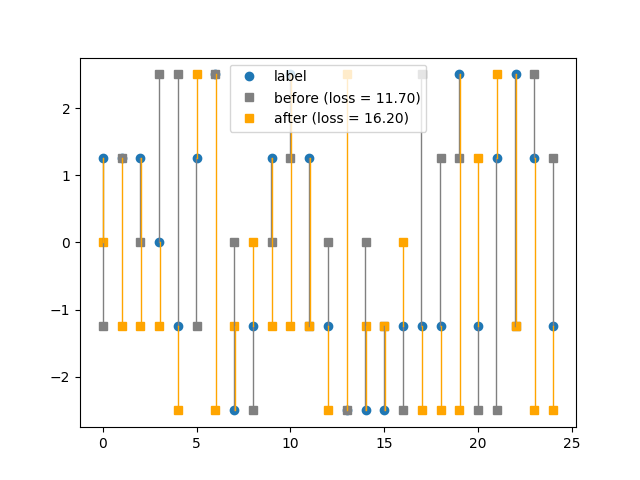
\includegraphics[width=0.4\linewidth]{xi0-1.png}
    \caption{Completely non-Markovian input, predicted and label states ($\xi$ = 0).}
    \label{fig:xi0-1}
    \end{figure}
\begin{figure}[H]
    \centering
    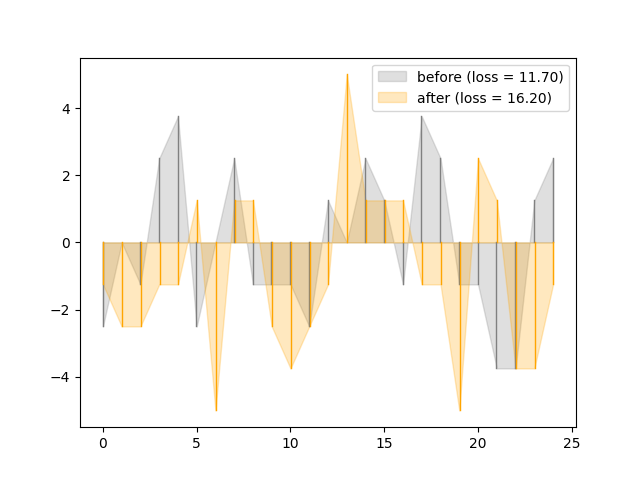
\includegraphics[width=0.4\linewidth]{xi0-2.png}
    \caption{Completely non-Markovian input and predicted label differences ($\xi$ = 0).}
    \label{fig:xi00-2}
\end{figure}

\begin{figure}
    \centering
    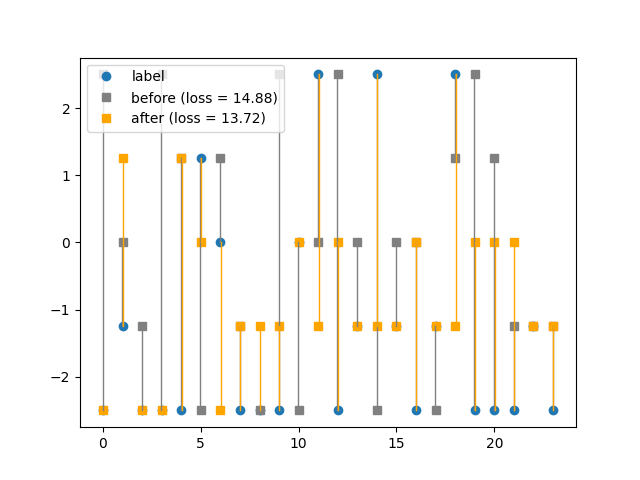
\includegraphics[width=0.5\linewidth]{xi05-1.png}
    \caption{Partially non-Markovian input, predicted and label states ($\xi$ = 0.5).}
    \label{fig:xi05-1}
\end{figure}
\begin{figure}
    \centering
    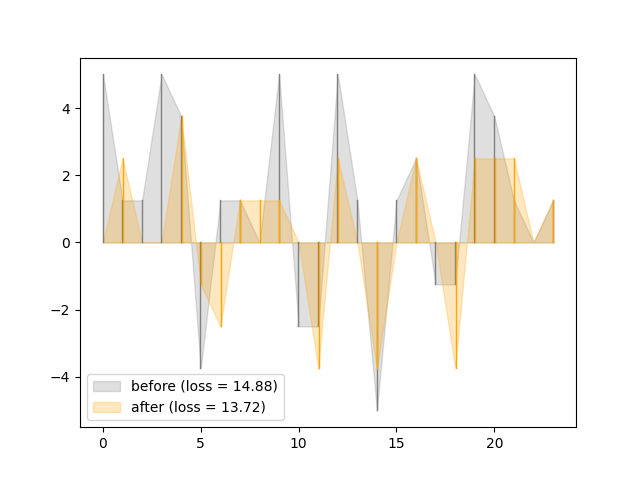
\includegraphics[width=0.5\linewidth]{xi05-2.png}
    \caption{Partially non-Markovian input and predicted label differences ($\xi$ = 0.5).}
    \label{fig:xi05-2}
\end{figure}

\begin{figure}
    \centering
    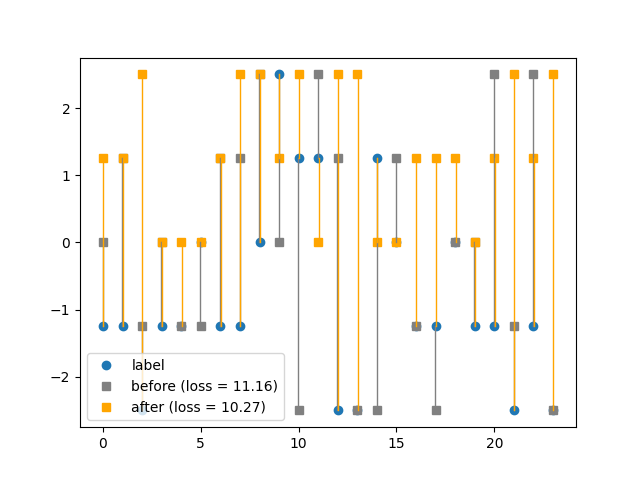
\includegraphics[width=0.5\linewidth]{xi1-1.png}
    \caption{Completely Markovian input, predicted and label states ($\xi$ = 1).}
    \label{fig:xi10-1}
\end{figure}
\begin{figure}
    \centering
    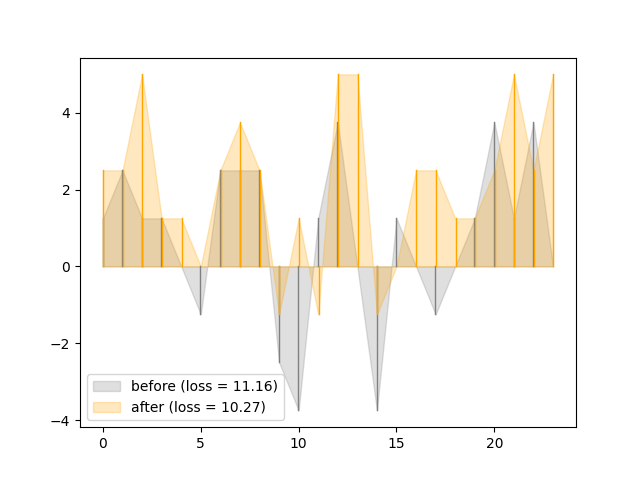
\includegraphics[width=0.5\linewidth]{xi1-2.png}
    \caption{Completely Markovian input and predicted label differences ($\xi$ = 1).}
    \label{fig:xi10-2}
\end{figure}

Each trial took approximately 5 hours to run.  

Final loss  decrease as the source becomes more Markovian. However, the variation between the initial dataset losses show that the difference between the original loss and the final loss is highest (even increases after training) in the completely non-Markovian case, but remains relatively unchanging between the partially non-Markovian and completely Markovian case. 


Several other thoughts from the past experiement are below: 
\begin{itemize}
    \item The control doesn't have enough degrees of freedom to model the generating process
        
    \begin{itemize}
        \item The generating process is too complicated with random matrices. Could opt for something less general, more simple. 
        \item The action space (m-quantized) is too small. (unfortunately, dependency on m is exponential)
    \end{itemize}

    \item The generating process is flawed by design. Since I'm averaging long-term dependencies for the non-Markovian transition probability, it might actually provide more stability than its Markovian counterpart. I could simply replace P2 (which captures long term dependency) with iid noise, as you've suggested. 

    \item The state space (n-quantized) is too small. Doesn't efficiently pass information between layers.

    \item Markovian actually does improve loss in general. This small trial might not be indicative. 

\end{itemize}


Note: in the cases of inputs multiple labels, I don't show the entire label distribution, only the most common. Difficult to show the entire distribution without overcrowding, but I'll fix this for accuracy in the future. I also realize I didn't add axes labels, I'll fix that.

Here's the updated prediction vs actual display:

\begin{figure}
    \centering
    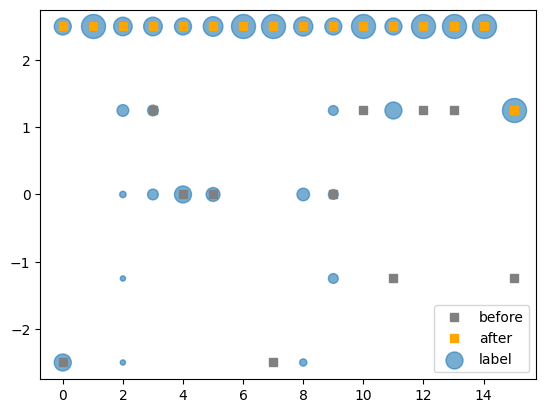
\includegraphics[width=0.5\linewidth]{example_display.png}
    \caption{Updated display. The radius of the label circle corresponds to occurrences in the distribution}
    \label{fig:placeholder}
\end{figure}

% \section{Next steps}
% 
% Edits:
% \begin{itemize}
%     \item Previous probability measures and quantization was redundant. Since N is known, there's no point dividing the dirac measure by N, and then quantizing it so that the entire 'prompt' has measure 1 and each token has measure 1/N. Instead, each token has measure 1 and the prompt has measure N; therefore, quantization with $R_l$ is no longer needed for x, only for y. 
% \end{itemize}

\newpage
\bibliographystyle{plain}
\bibliography{References}

\end{document}
